% !TeX root = ../../tesi.tex

RT-DETR (Real-Time Detection Transformer) extends the DETR paradigm toward real-time object detection by preserving its end-to-end formulation while explicitly addressing the latency and computational limitations that hindered earlier transformer-based detectors \cite{zhao_detrs_2024}. As in DETR, object detection is formulated as a set prediction problem, so that the model directly outputs a fixed set of detections without relying on heuristic post-processing such as Non-Maximum Suppression (NMS). The main contribution of RT-DETR lies in making this formulation practical for real-time scenarios.
\begin{figure}[h]
    \centering
    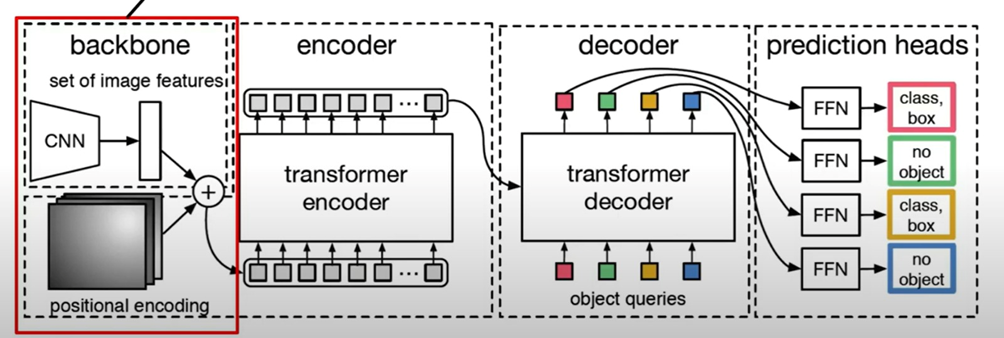
\includegraphics[scale=0.7]{images/DETR.png}
    \caption{Original DETR architecture.}
    \label{fig:DETR_architecture}
\end{figure}

From an architectural perspective, RT-DETR retains the standard backbone--encoder--decoder structure of DETR-style detectors, with prediction heads for object classification and bounding box regression. In this pipeline, the encoder is responsible for processing and fusing the visual features extracted by the backbone, so as to build a more informative representation of the scene before object queries are introduced. The decoder then takes these encoded features together with a set of object queries and iteratively refines them into final detections, progressively improving class predictions and bounding box localization. However, RT-DETR introduces several refinements designed to improve the accuracy--speed trade-off. In particular, the model employs an \textbf{efficient hybrid encoder} to process multi-scale visual features more efficiently by decoupling intra-scale interaction from cross-scale fusion \cite{zhao_detrs_2024}. This design reduces the computational burden of the encoder while still preserving the multi-scale information required for object detection.

\begin{figure}[h]
    \centering
    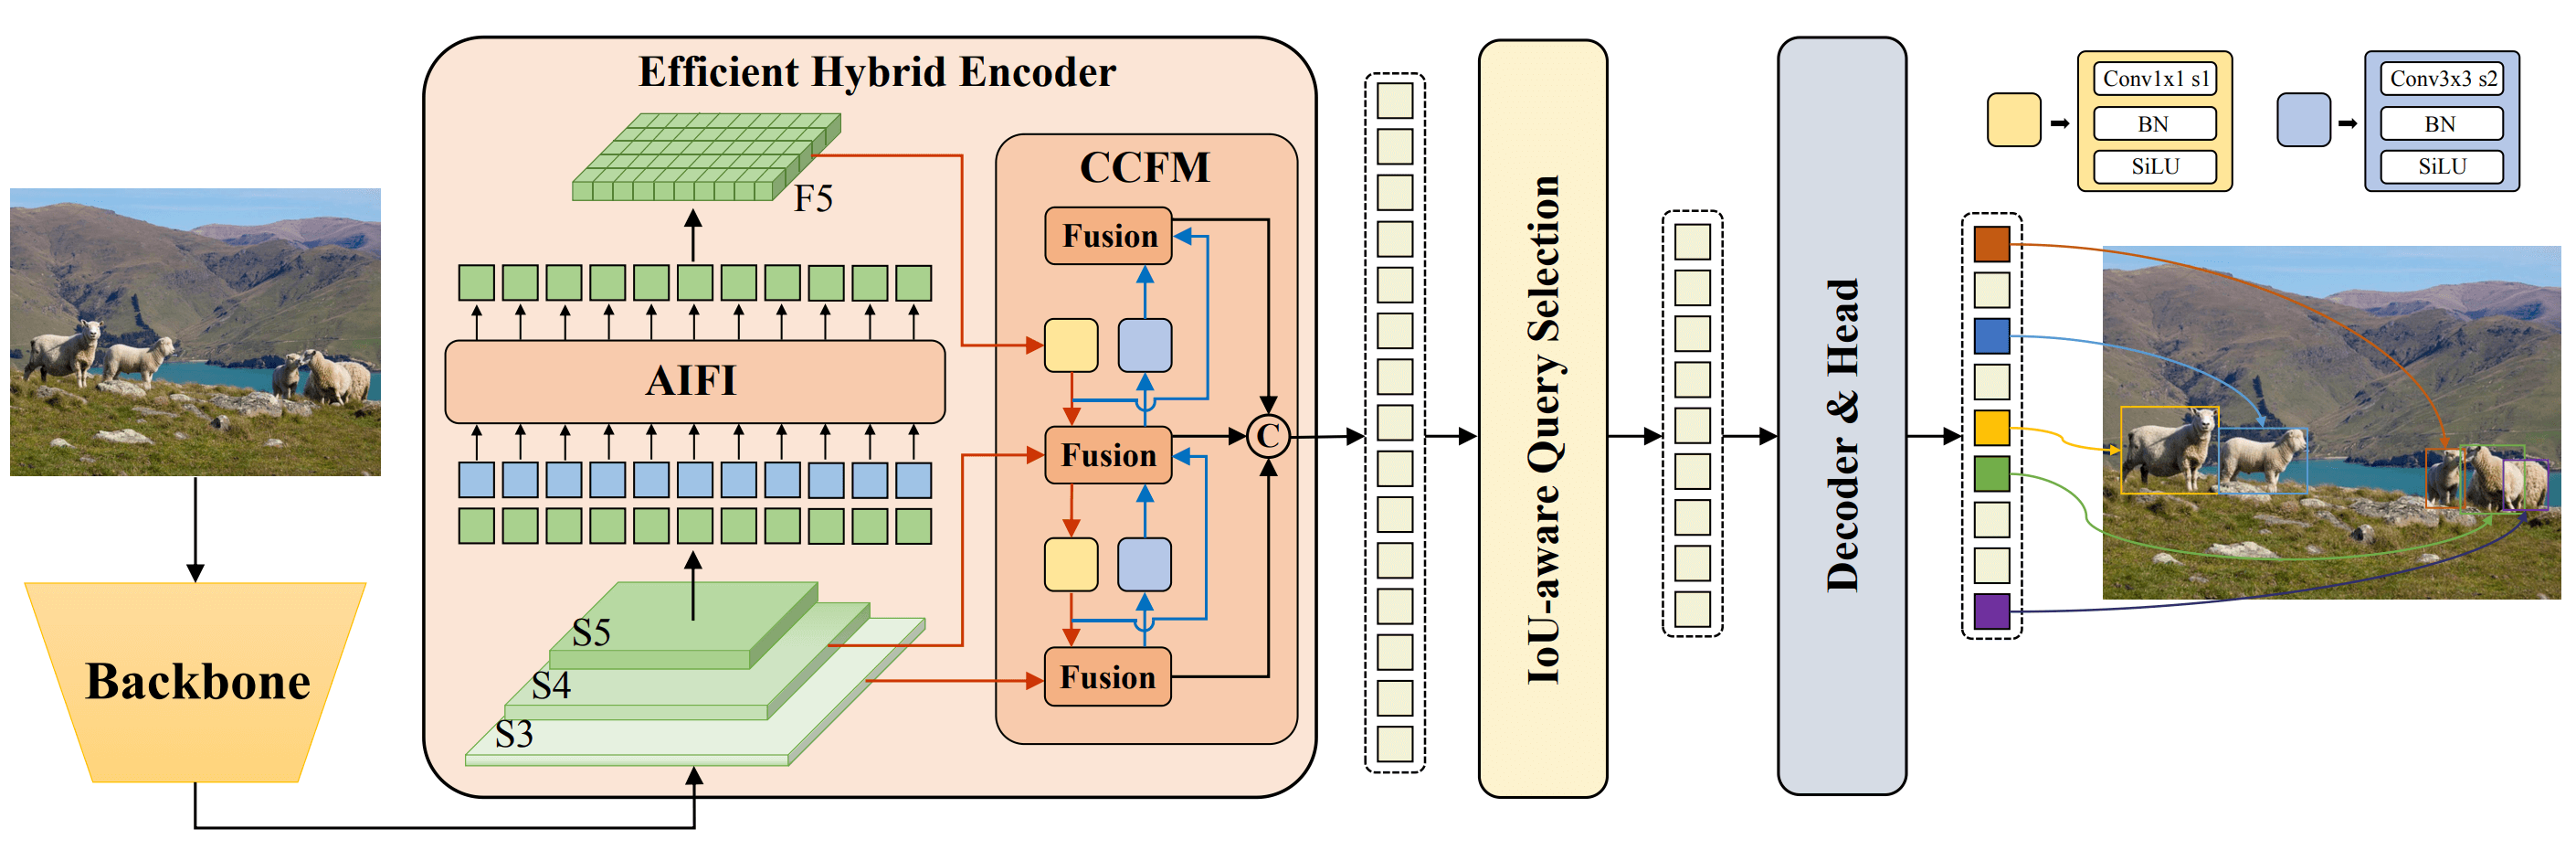
\includegraphics[scale=0.15]{images/RT-DETR.png}
    \caption{RT-DETR architecture.}
    \label{fig:RT-DETR_architecture}
\end{figure}

Another distinctive component is the \textbf{uncertainty-minimal query selection} strategy proposed to initialize the decoder with higher-quality object queries \cite{zhao_detrs_2024}. Rather than forwarding a large set of generic queries, RT-DETR selects encoder features that are expected to be more reliable starting points for detection. Intuitively, the model favors features that are informative both for object classification and for localization, so that the decoder begins its refinement process from more promising candidate regions. This improves efficiency and contributes to stronger detection accuracy.

This query selection mechanism should not be interpreted as a simple hand-crafted thresholding rule, such as selecting all predictions above a fixed IoU value. Instead, it is part of the learned initialization process of the detector and is designed to provide the decoder with a compact set of high-quality queries. After this initialization, the decoder iteratively refines the selected queries into final predictions.

In addition, RT-DETR retains the one-to-one matching paradigm based on the \textbf{Hungarian algorithm}, ensuring that each predicted object is assigned to at most one ground-truth instance during training. This bipartite matching mechanism is central to DETR-style detectors because it removes duplicate assignments and enables an end-to-end detection pipeline without NMS \cite{zhao_detrs_2024}.
\begin{figure}[h]
    \centering
    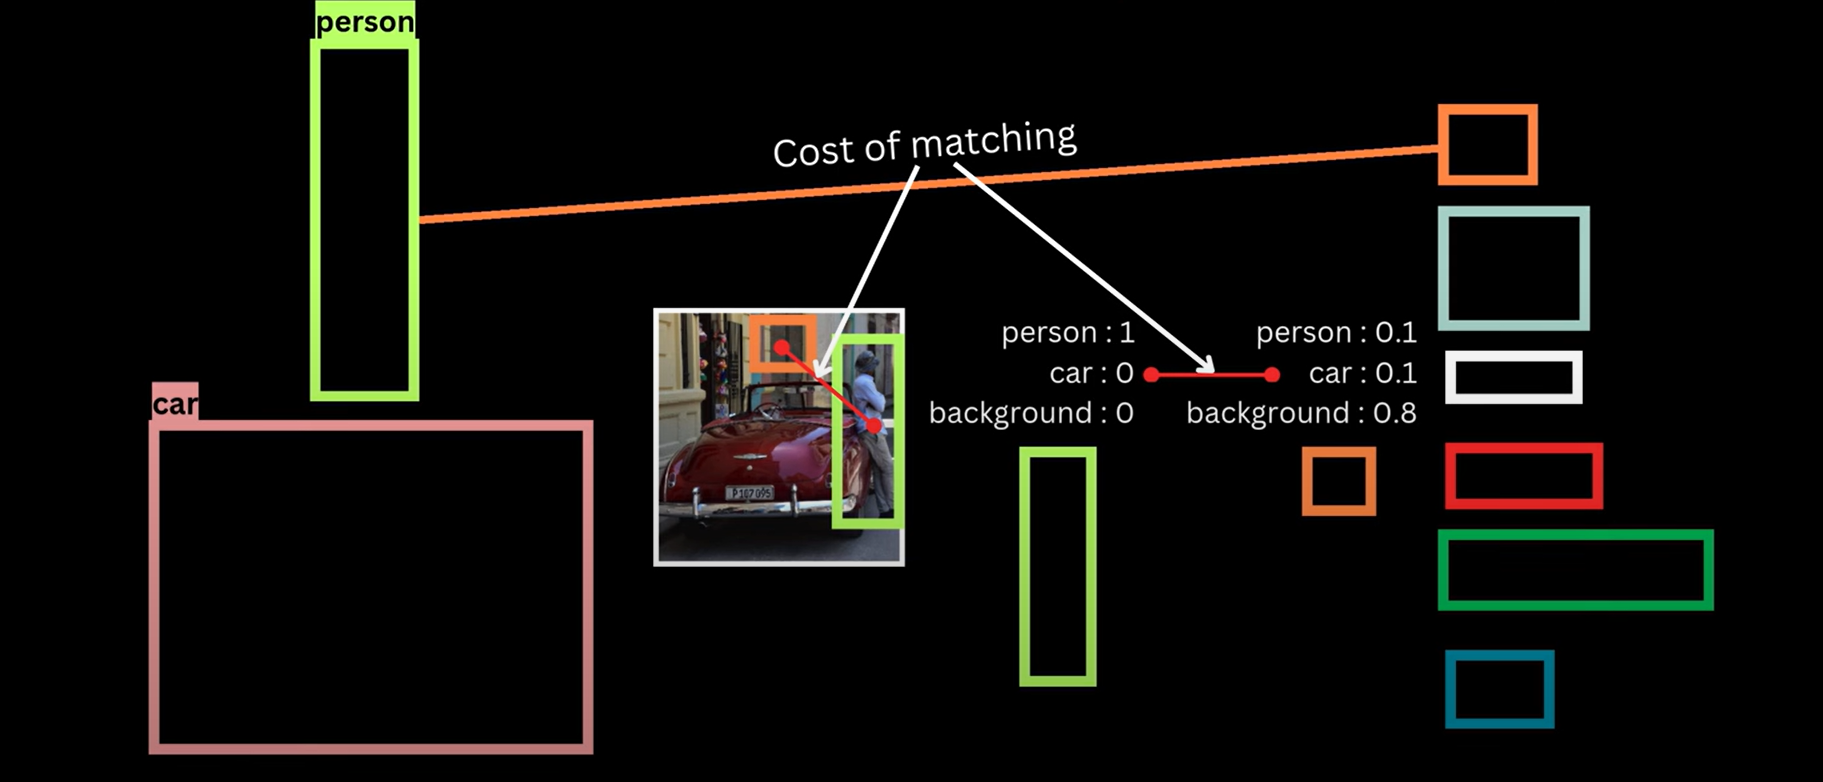
\includegraphics[scale=0.2]{images/Hungarian_match.png}
    \caption{Hungarian matching in RT-DETR.}
    \label{fig:Hungarian_match}
\end{figure}

An additional practical advantage of RT-DETR is its \textbf{flexible speed tuning}: the inference speed can be adjusted by varying the number of decoder layers, allowing the model to adapt to different deployment constraints without retraining \cite{zhao_detrs_2024}. Overall, RT-DETR achieves a strong balance between detection accuracy and computational efficiency, making transformer-based object detection more compatible with real-time and resource-constrained applications. In the context of this thesis, RT-DETR is particularly relevant because it shows how transformer principles can be adapted from generic vision representation learning to an efficient end-to-end detector, while also providing the conceptual basis for subsequent models such as DEIMv2.
